\documentclass[11pt,a4paper]{article}
\usepackage{ngerman}
\usepackage{hyperref}
\usepackage{graphicx}
\usepackage[paper=a4paper,left=25mm,right=25mm,top=25mm,bottom=25mm]{geometry}
\begin{document}

\title{EPR Übungsblatt Nr.7 - Dokumentation}
\author{6601128, Schademan, 7232927, Tobias}
\maketitle

\section*{Annahmen}
\begin{enumerate}
\item[•] Spieler schießen stets auf das Feld des jeweils danach schießenden Spielers.
\item[•] Es ist möglich, dass man Schiffe direkt nebeneinander platziert.
\item[•] Wenn ein Spieler aufgibt, ist das Spiel nicht beendet, sondern wird unter den verbleibenden Spielern fortgeführt. Sollte danach nur noch ein Spieler übrig sein, endet das Spiel natürlich.
\item[•] Wenn während eines Zuges die Zeit abläuft, ist der nächste Spieler an der Reihe.
\item[•] Das Spiel ist über den GameManager zu starten.
\end{enumerate}

\section*{Symbole}
\begin{enumerate}
\item[]
\includegraphics[width=5mm]{ship.PNG} steht für ein Schiff.
\item[]
\includegraphics[width=5mm]{ship_hit.PNG} steht für ein getroffenes Schiff.
\item[]
\includegraphics[width=5mm]{water.PNG} steht für Wasser.
\item[]
\includegraphics[width=5mm]{water_hit.PNG} steht für getroffenes Wasser.
\end{enumerate}


\section*{Aufwandseinschätzung}
Die Erstellung der GUI an sich stellte kein großes Problem dar, jedoch hat sich das Management der einzelnen Frames (also in unserem Fall die verschieden darstellbaren Möglichkeiten des Bildschirms) als eine recht aufwändige Arbeit erwiesen. Ohne vorherige Erfahrung mit TkInter kam es sehr häufig vor, dass einzelne Elemente mehrfach auf dem Bildschirm erschienen sind.\\\\
Da wir das Spielfeld aus einer Menge von Buttons erstellt haben, musste zunächst auch herausgefunden werden, wie es möglich ist, die jeweilige Position als Parameter zu übergeben (lambda). Durch dieses mangelnde Wissen konnten wir die Arbeitsabläufe im Vorhinein nicht ganz richtig einschätzen, weshalb wir recht schnell recht viel von unserem ursprünglichen Konzept abweichen mussten und dieses immer wieder angepasst haben.\\\\
Wenn ein Spieler schießt, dann wird auf dem Bildschirm nicht nur sein eigenes Feld angezeigt, sondern auch das des Gegners. Wenn dann diese Phase vorbei ist, müssen beide Spieler instruiert werden, ihr Feld auszublenden. Dabei muss auch darauf geachtet werden, dass danach der richtige Grund angezeigt wird, weshalb die Runde beendet wurde (Timeout, daneben geschossen, usw.). Die Implementierung dieses Vorgangs war am aufwändigsten, da dabei viele Informationen zwischen verschiedenen Instanzen verschiedener Klassen ausgetauscht werden müssen.\\\\
Beim nächsten mal ist ein besseres Wissen über TkInter vorhanden, weshalb sich bei der anfänglichen Konzeption darauf besser eingehen lässt. Dadurch kann man vorher besser Planen und muss nicht während des Programmieren andauernd Anpassungen vornehmen.

\section*{Zustandsdiagramm}
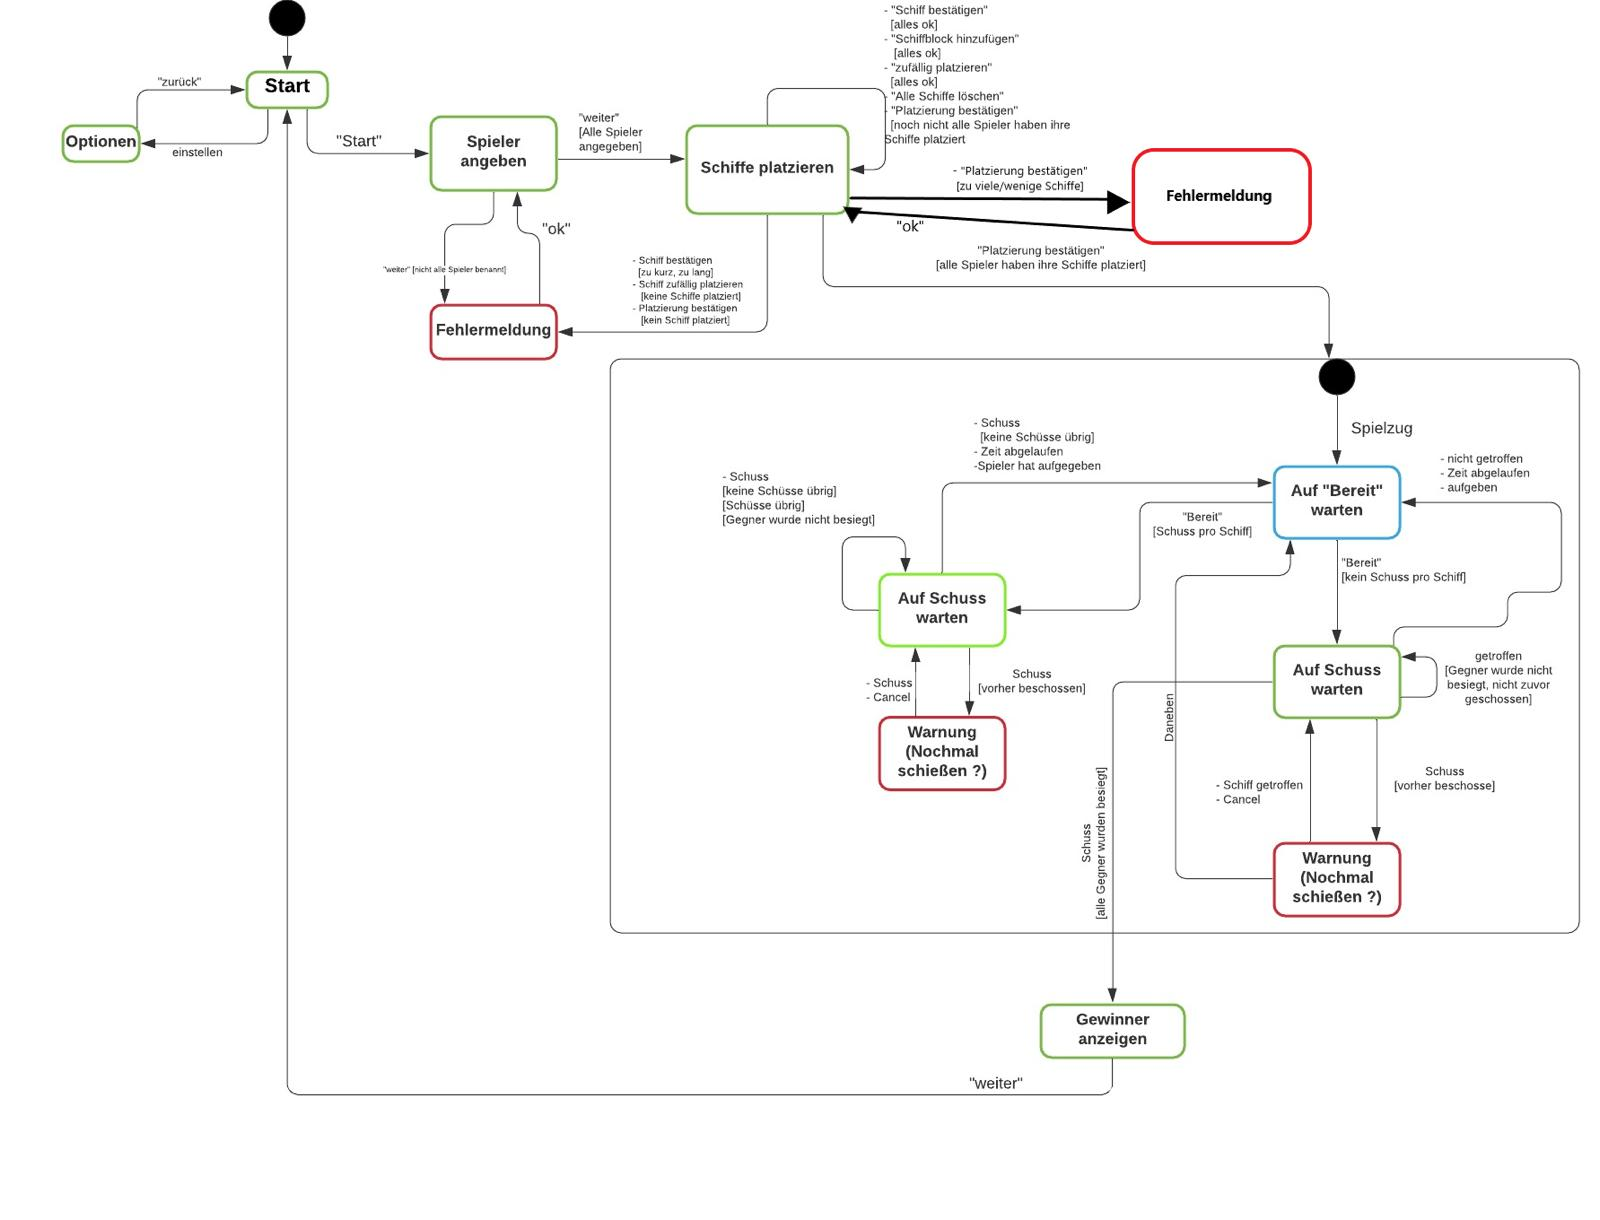
\includegraphics[width=17cm]{uml.jpg}

\end{document}